\documentclass[12pt]{article}
\usepackage[a4paper, portrait, margin=1cm, bottom=2cm]{geometry}
\usepackage{fontspec}
\usepackage[fleqn]{amsmath}
\usepackage{indentfirst}
\usepackage{graphicx}
\usepackage{framed}

\setmainfont[Ligatures=TeX]{Linux Libertine}
\graphicspath{./graphics/}

\title{АиГ. ДЗ к 2023-05-25. Кривые второго порядка. Вариант №14}
\author{Студент группы 2305 Александр Макурин}
\date{25 мая 2023}

\begin{document}
\maketitle
\section{Привести уравнение кривой второго порядка к каноническому виду, найти координаты центра и фокусов в исходной системе координат и построить эскиз графика: $9x^2 - 6y^2 + 8xy + 34x - 16y = 69$.}
\[
    A = \begin{pmatrix}
        9 & 4  \\
        4 & -6 \\
    \end{pmatrix} \\
    B = \begin{pmatrix}
        9 - \lambda & 4            \\
        4           & -6 - \lambda \\
    \end{pmatrix} \\
    |B| = \lambda^2 - 3\lambda - 70
\]
\[
    \lambda_{1,2} = -7; 10
\]
\[
    \lambda = 10: \begin{pmatrix}
        -1 & 4   \\
        4  & -16 \\
    \end{pmatrix} \sim \begin{pmatrix}
        1 & -4 \\
        0 & 0  \\
    \end{pmatrix}
    \Rightarrow x = 4y \\
    t_1\begin{pmatrix} 4 \\ 1 \end{pmatrix}
\]
\[
    \lambda = -7: \begin{pmatrix}
        16 & 4 \\
        4  & 1 \\
    \end{pmatrix} \sim \begin{pmatrix}
        4 & 1 \\
        0 & 0 \\
    \end{pmatrix}
    \Rightarrow 4x = -y \\
    t_2\begin{pmatrix} 1 \\ -4 \end{pmatrix}
\]
\[
    C = \dfrac{1}{\sqrt{17}}\begin{pmatrix}
        4 & 1  \\
        1 & -4 \\
    \end{pmatrix} \\
    C^{-1} = C^T = C = \dfrac{1}{\sqrt{17}} \begin{pmatrix}
        4 & 1  \\
        1 & -4 \\
    \end{pmatrix}
\]
\[
    \begin{cases}
        x = \dfrac{4x' + y'}{\sqrt{17}} \\
        y = \dfrac{x' - 4y'}{\sqrt{17}}
    \end{cases}
    \\
    \begin{cases}
        x' = \dfrac{4x + y}{\sqrt{17}} \\
        y' = \dfrac{x - 4y}{\sqrt{17}}
    \end{cases}
\]
\[
    \dfrac{9}{17}(4x' + y')^2 - \dfrac{6}{17}(x' - 4y')^2 + \dfrac{8}{17}(4x' + y')(x' - 4y') + 2\sqrt{17} (4x' + y') - \dfrac{16}{\sqrt{17}}(x' - 4y') = 69 \\
\]
\[
    9(16{x'}^2 + 8x'y' + {y'}^2) - 6({x'}^2 - 8x'y' + 16{y'}^2) + 8(4{x'}^2 - 15x'y' - 4{y'}^2) + 34\sqrt{17}(4x' + y') - 16\sqrt{17}(x' - 4y') = 1173
\]
\[
    (144 - 6 + 32){x'}^2 + (72 + 48 - 120)x'y' + (9 - 96 - 32){y'}^2 + 120\sqrt{17}x' + 98\sqrt{17}y' - 1173 = 0
\]
\[
    (\sqrt{17}\sqrt{10}{x'})^2 + 2 \cdot 6 \sqrt{10} \sqrt{10} \sqrt{17}x' - ((\sqrt{17}\sqrt{7}{y'})^2 - 2 \cdot 7 \sqrt{7} \sqrt{7} \sqrt{17}y') - 1173 = 0
\]
\[
    170({x'} + \dfrac{6}{\sqrt{17}})^2 - 360 - 119({y'} - \dfrac{7}{\sqrt{17}})^2 + 343 - 1173 = 0
\]
\[
    \begin{cases}
        x'' = x' + \dfrac{6}{\sqrt{17}} \\
        y'' = y' - \dfrac{7}{\sqrt{17}}
    \end{cases}
    \\
    \begin{cases}
        x' = x'' - \dfrac{6}{\sqrt{17}} \\
        y' = y'' + \dfrac{7}{\sqrt{17}}
    \end{cases}
\]
\[
    170{x''}^2 - 119{y''}^2 = 1190 \ \ \ \ | : 1190
\]
\[
    \dfrac{x''}{\sqrt{7}}^2 - \dfrac{y''}{\sqrt{10}}^2 = 1 \text{ — гипербола}
\]

В системе координат $x'', y''$ гипербола имеет следующие параметры:
\[
    C(0, 0) \\ F_{1,2}(\pm\sqrt{17}, 0)
\]

В системе координат $x', y'$:
\[
    C(-\dfrac{6}{\sqrt{17}}, \dfrac{7}{\sqrt{17}}) \\ F_{1,2}\left(\dfrac{\pm 17 - 6}{\sqrt{17}}, \dfrac{7}{\sqrt{17}}\right)
\]

В исходной системе координат $x, y$:
\[
    C(-1, -2) \\ F_{1,2} = (-1, -2) \pm (4, 1)
\]

\begin{framed}
    Ответ: гипербола с координатами центра $C(-1, 2)$, фокусов $F_1(-5, -3)$ и $F_2(3, -1)$. График:\\
    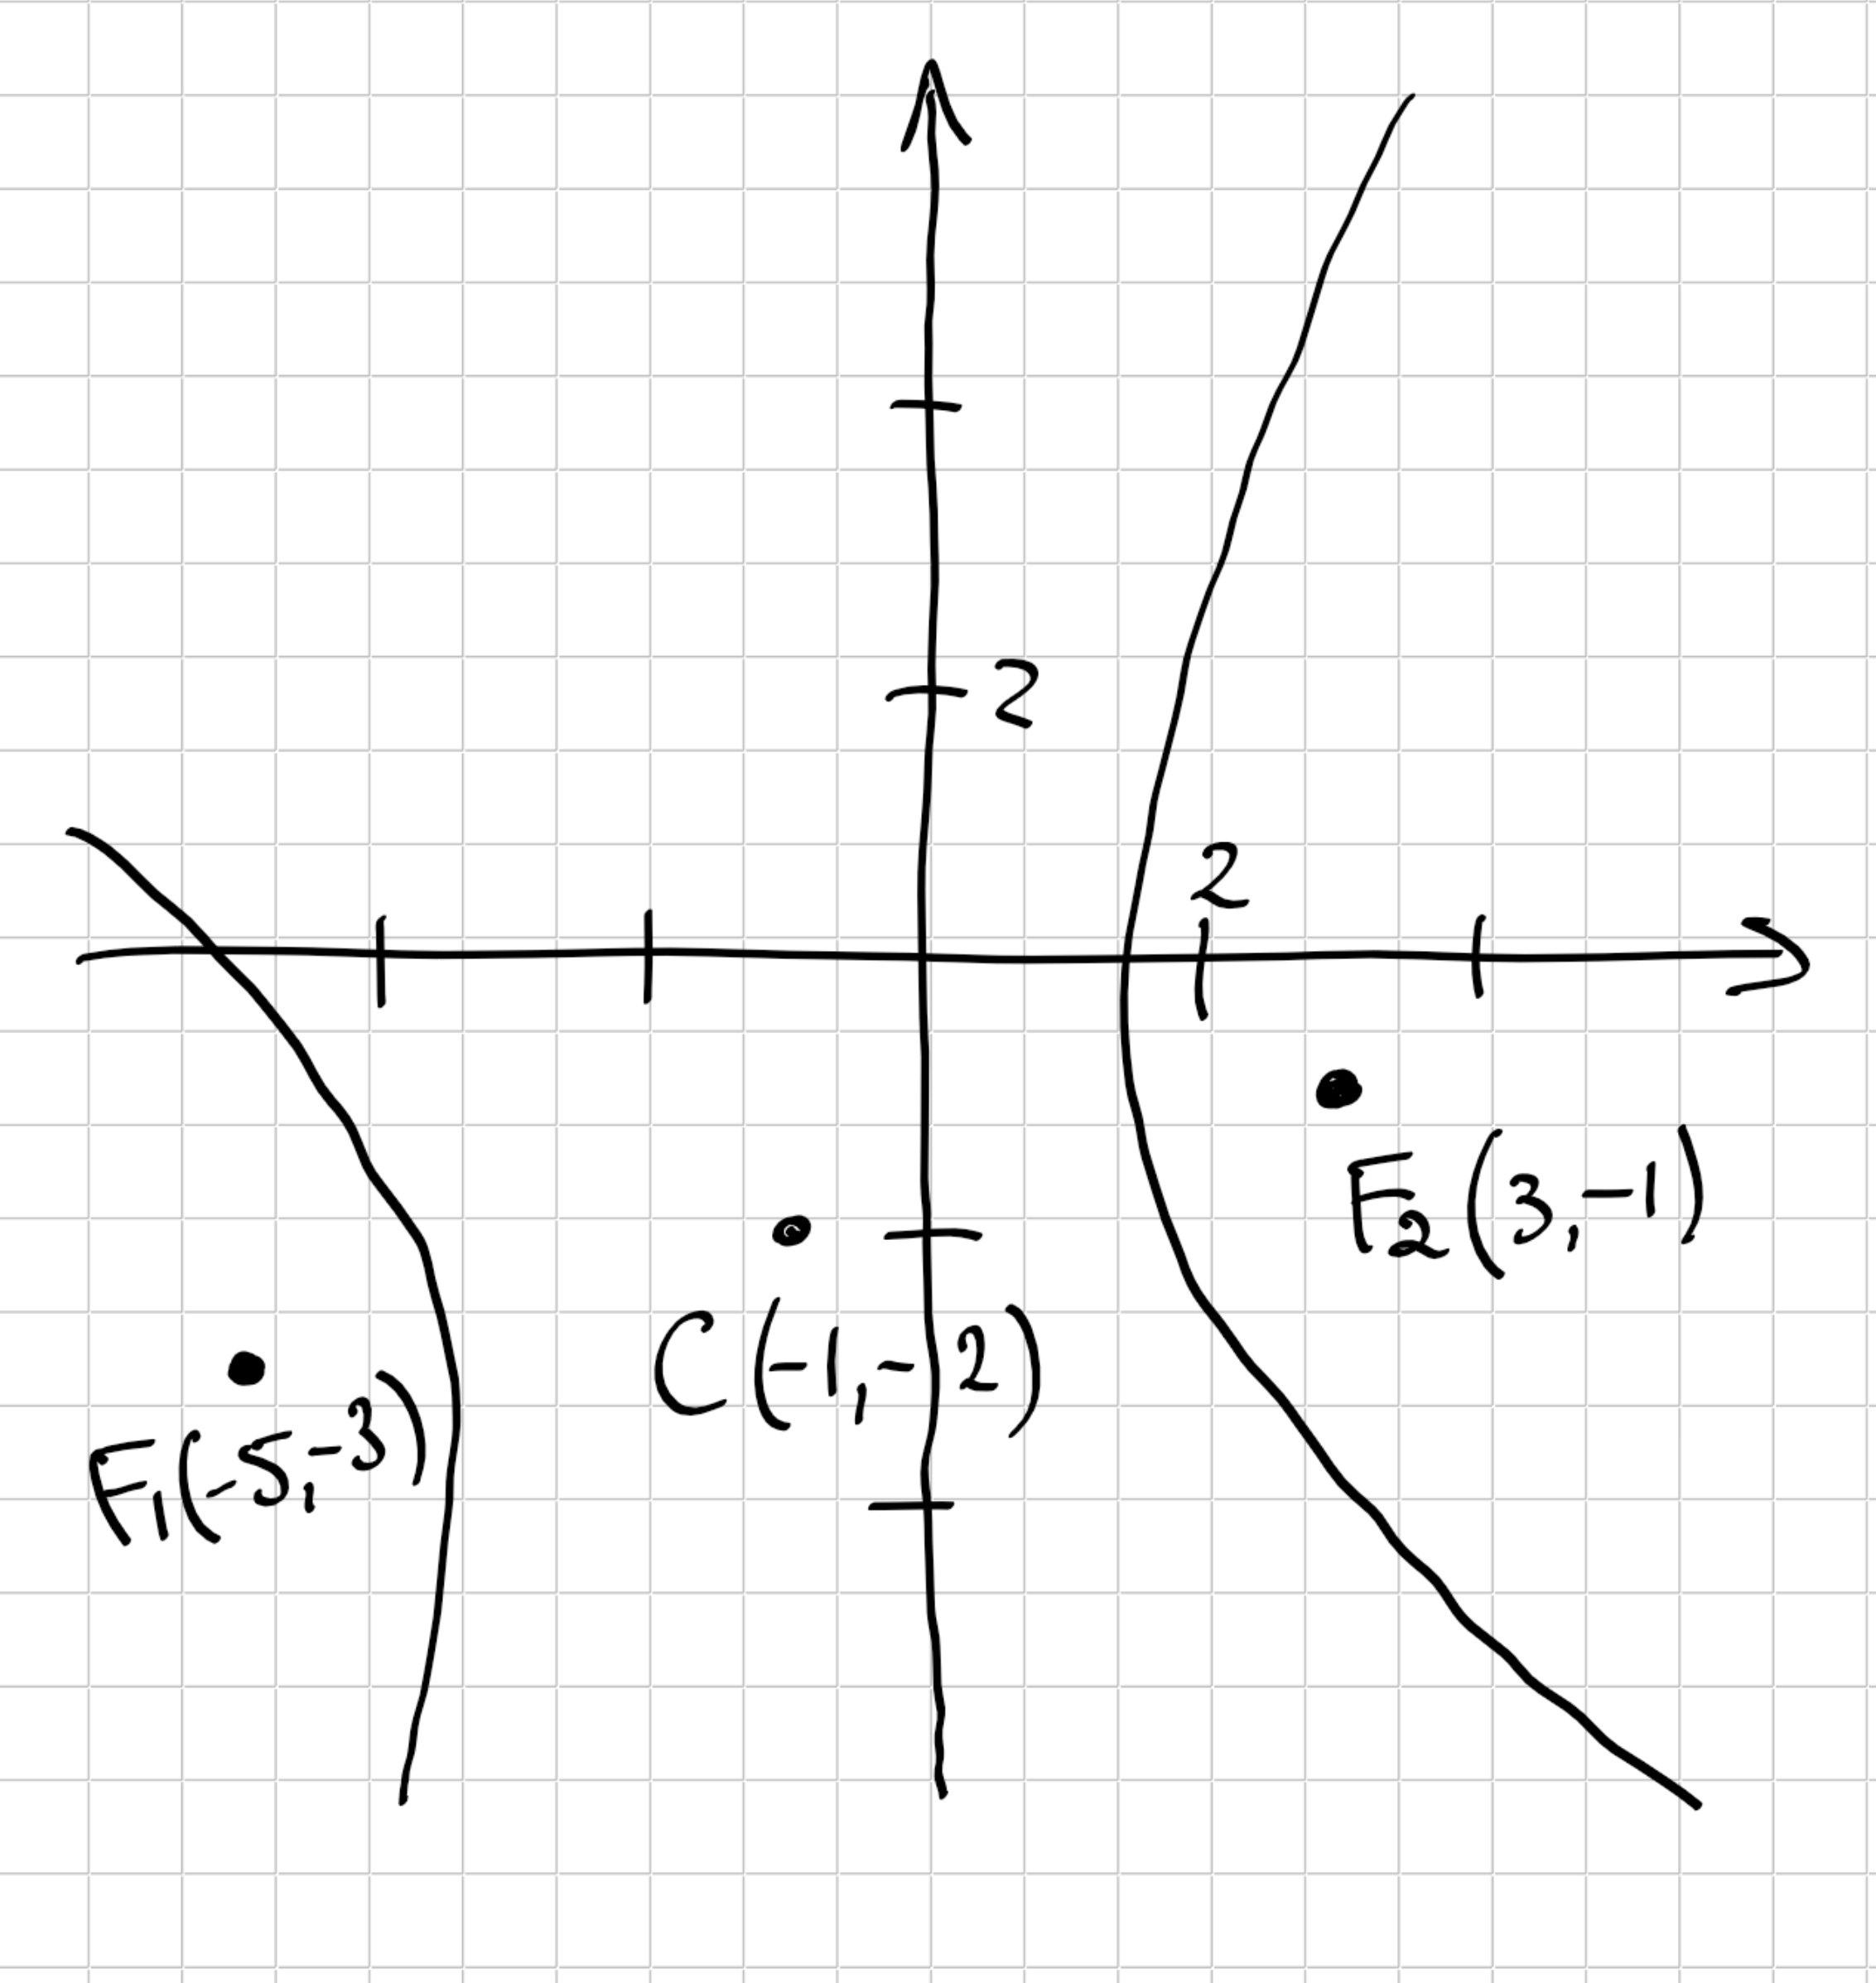
\includegraphics[width=0.5\textwidth]{./graphics/menshe.png}
\end{framed}

\section{Определить тип поверхности второго порядка и найти координаты её центра (если он существует): $x^2 + 2y^2 + 4z^2 + 6xy - 12xz - 6yz - 4x + 2y - 6z = 3$}
\[
    x^2 + 2y^2 + 4z^2 + 6xy - 12xz - 6yz - 4x + 2y - 6z = 3
\]
\begin{align*}
     & x^2 + 2y^2 + 4z^2 + 6xy - 12xz - 6yz = x^2 + 2x (3y - 6z) + (9y^2 - 36yz + 36z^2) - 7y^2 + 30yz - 32z^2 = \\
     & = (x + (3y - 6z))^2 - 7y^2 + 30yz - 32z^2
\end{align*}
\[
    (x + (3y - 6z))^2 - (7y^2 - 30yz + 32z^2) - 4x + 2y - 6z = 3
\]
\begin{align*}
     & 7y^2 - 30yz + 32z^2 = 7(y^2 - 2 \cdot \dfrac{15}{7}yz + \dfrac{32}{7}z^2) = 7(y - \dfrac{15}{7}z)^2 - \dfrac{1}{7}z^2
\end{align*}
\[
    (x + (3y - 6z))^2 - 7(y - \dfrac{15}{7}z)^2 + \dfrac{1}{7}z^2 - 4x + 2y - 6z = 3
\]
\[
    \begin{cases}
        x' = x + 3y - 6z        \\
        y' = y - \dfrac{15}{7}z \\
        z' = z
    \end{cases}
    \\
    \begin{cases}
        x = x' - 3y' - \dfrac{45}{7}z' + 6z' = x' - 3y' - \dfrac{3}{7}z' \\
        y = y' + \dfrac{15}{7}z'                                         \\
        z = z'
    \end{cases}
\]
\begin{align*}
     & -4x + 2y - 6z = -4x' + 12y - 24z + 2y - 6z = -4x' + 14y - 30z = -4x' + 14y'
\end{align*}
\[
    {x'}^2 - 7{y'}^2 - \dfrac{1}{7}{z'}^2 - 4x' + 14y' = 3
\]
\[
    ({x'}^2 - 2 x'\cdot 2 + 4) - 4 - 7({y'}^2 - 2 y' \cdot 1 + 1) + 7 + \dfrac{1}{7}{z'}^2 = 3
\]
\[
    \begin{cases}
        x'' = x' - 2 \\
        y'' = y' - 1 \\
        z'' = z'
    \end{cases}
    \\
    \begin{cases}
        x' = x'' + 2 \\
        y' = y'' + 1 \\
        z' = z''
    \end{cases}
\]
\[
    {x''}^2 - 7{y''}^2 + \dfrac{1}{7}{z''}^2 = 0 \text{ — конус}
\]

Центр в системе координат $x'', y'', z''$ находится в точке $C(0, 0, 0)$.

В системе координат $x', y', z'$: $C(2, 1, 0)$.

В системе координат $x, y, z$: $C(-1,1,0)$.

\fbox{Ответ: действительный конус с центром в точке $C(-1, 1, 0)$}
\end{document}